\chapter{Konzeption und Methodik}


Das Konzept dieser Arbeit ist auf 3 Säulen aufgebaut. Erstens, das Sammeln, Speichern und Analyse der Daten und die Analyse der Daten, zweitens, das Entwickeln eines Deep Learning Modells, welches durch die gesammelten und angepassten Daten entsteht und drittens, das Implementieren und Einbetten des Modells in eine Benutzeroberfläsche, also in die Clientseite, siehe Abbildung~\ref{Kap5:Konzeption}.

\begin{figure}[H]
    \centering
    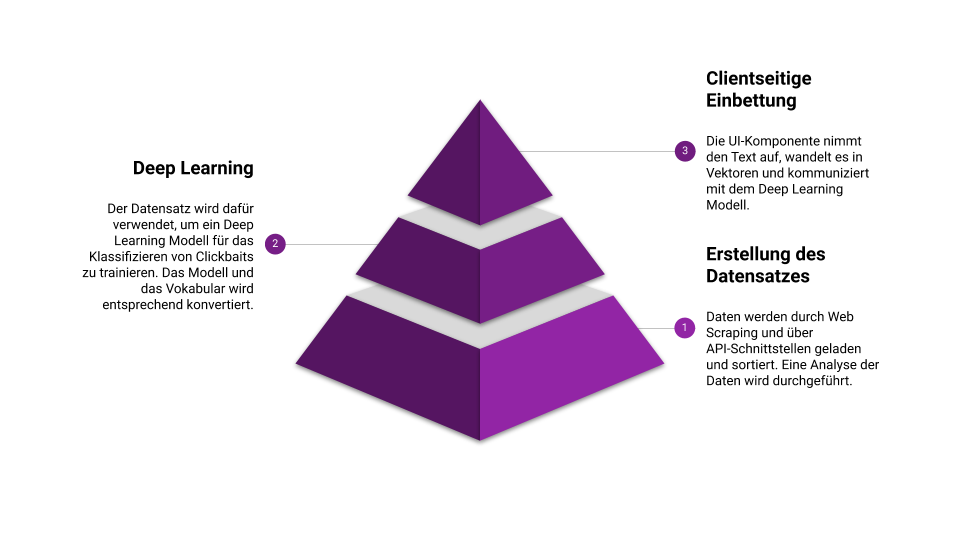
\includegraphics[width=15cm]{kapitel5/main_p.png}
    \caption[Darstellung der Konzeption]{Darstellung der Konzeption}
    \label{Kap5:Konzeption}
\end{figure}


Deep Learning Modelle benötigen eine große Menge an Beispielen um zu lernen. Es reicht außerdem nicht aus, nur eine große Menge an Daten zu beschaffen, sondern auch gute Daten auszuwählen. In der Studie von \cite*{Chakrabortya} haben die Autoren Daten aus dem Web geladen. Für die erste Kategorie, der Nicht-Clickbaits, wurde die Wikipedia-News-API verwendet. Um genug Beispiele für Clickbaits zu finden, sollten solche Medien herausgefunden werden. Um die Daten labeln zu können ist neben dem Titel eines Datenelementes auch die extraktion der Nachricht zu erfassen.

Die Wikipedia-News-API bietet einen Kostenlosen Endpunkt an, welches verschiedene Nachrichtenportale wie z.B. Politik, Wirtschaft, Kultur, Sport und Wissenschaft anbietet. Um Clickbaits zu finden verläuft die Datenaquise wesentlich schwieriger. Der Datensatz von \cite*{Chakrabortya} beinhalter jeweils 7500 Nachrichten je Kategorie. Es ist zu berücksichtigen, dass diese nicht mit Deep Learning Modellen arbeiten, sondern mit klassischen Machine Learning Algorithmen, die weniger Daten benötigen. Es müssen also mehr Daten her, also die Suche sollte neben den klassischen Clickbait-Seiten auch woanders erfolgen. Um die Datenextraktion zu automatisieren bietet sich die Software \enquote{Scrapy} an. Scrapy ist ein Open-Source Tool, welches das extrahieren von großen Mengen an Daten erleichtert. Es ist in Python geschrieben und kann durch seine Middleware Funktion auch die Daten direkt in eine SQL-Datenbank speichern.

Der mittlere Kern der Pyramide in Abbildung~\ref{Kap5:Konzeption} ist das Deep Learning Modell, welches als Inferenzmaschine betrachtet werden kann. Es wird durch Eingabe von gelabelten Daten trainiert und in ein entsprechendes Format gebracht. Es gibt mehrere Anbieter für das Deep Learning. Die meisten von Ihnen sind Open Source. Die bekanntesten Bibliotheken für das Deep Learning sind TensorFlow (welches von Google unterstützt wird) und PyTorch (welches von Facebook unterstützt wird). Seit März 2018 bietet TensorFlow die Möglichkeit, Modelle in der Programmiersprache JavaScript zu trainieren und zu benutzen. Ein klassischer Vorgang um Deep Learning Modelle dem Endbenutzer durch Webprogrammierung anzubieten war es immer, dass zunächst ein Modell trainiert wurde und dann auf einem Server geladen wurde. Der Server hatte dann einen Endpunkt, z.B. eine POST-Anfrage, welches eine Anfrage vom Clienten empfang. Diese Anfrage wurde dann im Server durch das Modell beantwortet und der Server sendete dem Clienten das Ergebnis. Durch TensorFlow.js ist es möglich erstens ein Modell komplett auf der Programmiersprache JavaScript zu entwickeln und zweitens es die Inferenzbildung durch einen Server in der Mitte nicht mehr nötig. Das Modell kann zusammen mit dem Framework in den Browser geladen werden und die bearbeitung erfolgt dort. In dieser Arbeit wurde das Modell nicht mit TensorFlow.js trainiert, da es auch möglich ist, Modelle in der konventionellen Weise mit der Keras API zu trainieren und dann in ein Webfreundliches Format umzuwandeln. Nach der Konversion können die Gewichte welches das Modell gerechnet hat und eine JSON-Datei, welches das Modell beschreibt hochgeladen und benutzt werden. Der Client muss nur noch diese Dateien in den Browser laden und kann dann selbst die Anfrage beantworten. Das trainieren auf konventionellen Wegen bietet außerdem den Vorteil, dass die Umgebung auf JavaScript nicht mit der Umgebung in Python konkurrieren kann. Die meisten Tools und Frameworks werden für Python geschrieben. Ein weiterer Grund ist, dass die bearbeitung auf dem heimischen Computer sehr langsam ist. Mit Google Colab können Deep Learning Modelle mit viel Rechnerkapazität trainiert werden.

Die Spitze der Pyramide macht die Benutzeroberfläsche aus. Diese wird komplett in JavaScript geschrieben. JavaScript ist die meistbenutze Programmiersprache und wird heute neben Webentwicklung auch auf dem Server verwendet. Mit TensorFlow.js ist es nun auch möglich, mit Tensors umzugehen. Die Schwierigkeit hier ist es, den Text, den der Benutzer eingibt, in Token und dann diese Token in Vektoren umzuwandeln, wenn das Modell keinen sogenannten \enquote{Input-Layer} hat welches einfache String einnehmen kann und diese umwandeln kann, dieses macht das Modell aber viel größer, da es eine größere Anzahl an Parametern hat und nicht Ziel dieser Arbeit. Eine andere Möglichkeit ist es, das gesamte Vokabular in einer JSON-Datei zu speichern und es der Benutzeroberfläsche zugänglich zu machen. Jedes auftauchende Wort im Vokabular bekommt einen Index, welches dann als \enquote{Übersetzer} dient und zur Umwandlung der Strings in Vektoren verwendet werden.